\section{Evaluation}




The overview of our evaluation results include:

\squishlist
    \item \textbf{Reducing end-to-end latency.} Because many intermediate steps are easier than end-to-end reasoning, many (up to 80\%) of the speculated steps are accepted. \name{} achieves a $1.4-3.0\times$ speedup over vanilla LRM inference. Additionally, when combined with speculative decoding, \name{} further reduces latency by $8.8-58.0\%$ over speculative decoding alone, highlighting the complementary nature of these optimizations.
    \item \textbf{Improving token-budget-aware accuracy.} Beyond latency reduction, \name{} also improves accuracy over the base model by $0.4-9.0\%$ under the same token budget. We empirically find that small, lightweight models typically have shorter output sequence lengths -- meaning, they need fewer thinking tokens before deriving an answer. Thus, by accepting many small model's speculated reasoning steps, \name{} reduces the token consumption compared to the base model's vanilla inference. When the token budget is low -- a common setup to curb inference cost and latency -- \name{} helps improve accuracy as the base model would need more tokens to get to an answer (Fig.~\ref{fig:acc_intuition}).
\squishend

\subsection{Setup}

\textbf{Models.} In our main results, we use two base models: QwQ-32B~\citep{qwq_32b} and Skywork-OR1-Preview-32B~\citep{skywork_32b}. We also use two different small models for speculation: DeepSeek-R1-1.5B~\citep{deepseek_r1} and Zyphra's ZR1-1.5B~\citep{zyphra_1.5b} -- both of which are based on Qwen-2.5~\citep{qwen2.5} and embed the capability of reasoning with long CoTs -- and evaluate all four different model combinations. We evaluate an additional base model with a different size and architecture, R1-70B~\citep{deepseek_r1}, a distilled version of DeepSeek-R1 onto Llama3.3-70B~\citep{llama3}, in~\S\ref{sec:70b_microbenchmark}.

\textbf{Datasets.} We evaluate \name{} on three diverse reasoning benchmarks: AIME~\citep{aime} for high-school competition-level mathematical problems, MATH500~\citep{math500} for high-school competition-level mathematical problems sampled from AMC 10, AMC 12, and AIME, and GPQA Diamond~\citep{gpqa} for graduate-level questions in general domains like biology, physics, and chemistry. The accuracy metric we evaluate on is pass@1. Similar to prior work~\citep{deepseek_r1}, we set k=16 when calculating pass@1 -- i.e., we generate 16 responses with temperature=0.6 for every query and calculate the average accuracy -- and set the token budget to be 8192 tokens to ensure an apples-to-apples comparison between baselines.  %

\textbf{Baselines.} We run vanilla inference using the small and base models as the latency and accuracy baseline, respectively. Aside from \name{}, we also run speculative decoding (``SpecDecode'') with the smaller model as the draft model, speculating five tokens at a time. To demonstrate \name{}'s compatibility with speculative decoding, we also run a ``\name{}+Decode'' baseline that employs the hierarchical speculation described in~\S\ref{sec:hierarchical_speculation}.

\textbf{Hardware.} We run our evaluations on two NVIDIA A6000-48GB GPUs. We use vLLM~\citet{vllm} 0.8.2 as the underlying inference engine and enable prefix caching. Both models are served with a tensor parallelism degree of two.  %



\begin{figure}[t]
    \centering
    \begin{subfigure}[b]{\textwidth}
        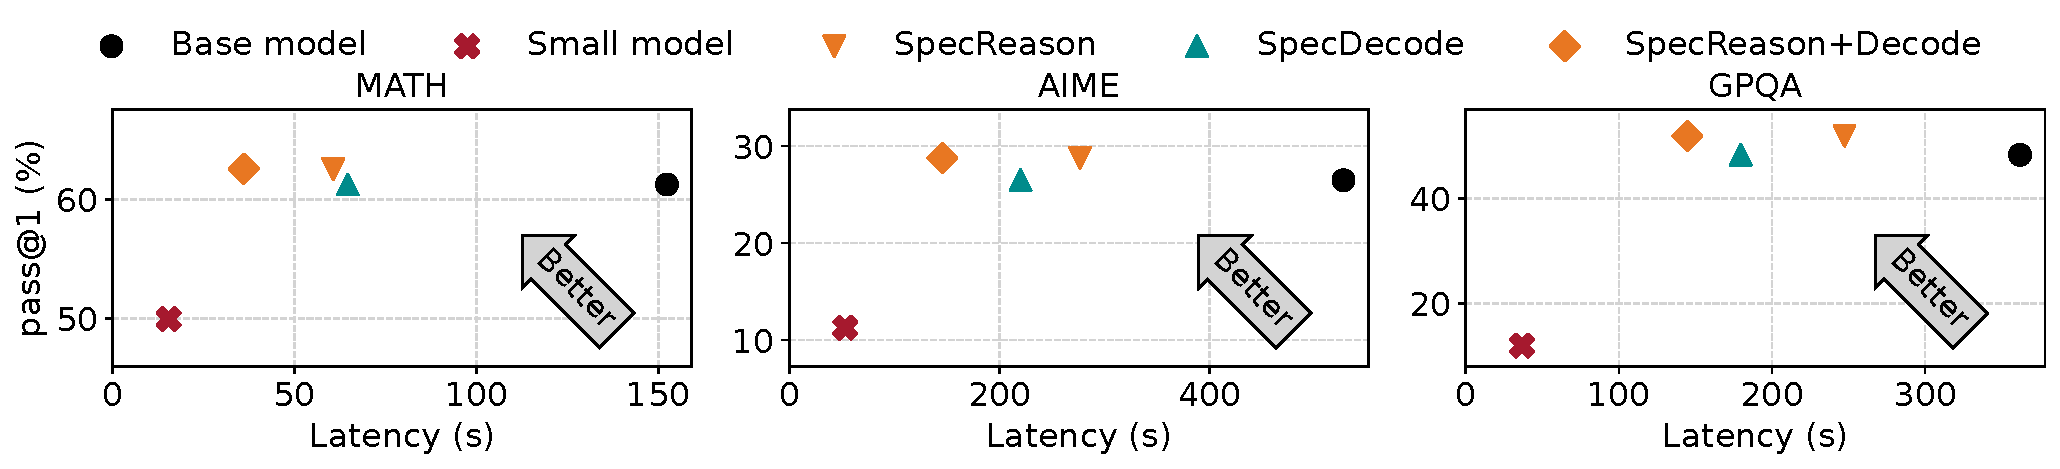
\includegraphics[width=0.99\textwidth]{figures/main_results/Qwen-32B_deepseek-1.5B.pdf}
        \vspace{-5pt}
        \caption{QwQ-32B + R1-1.5B}
        \label{fig:main_results_1}
    \end{subfigure}
    \hfill
    \begin{subfigure}[b]{\textwidth}
        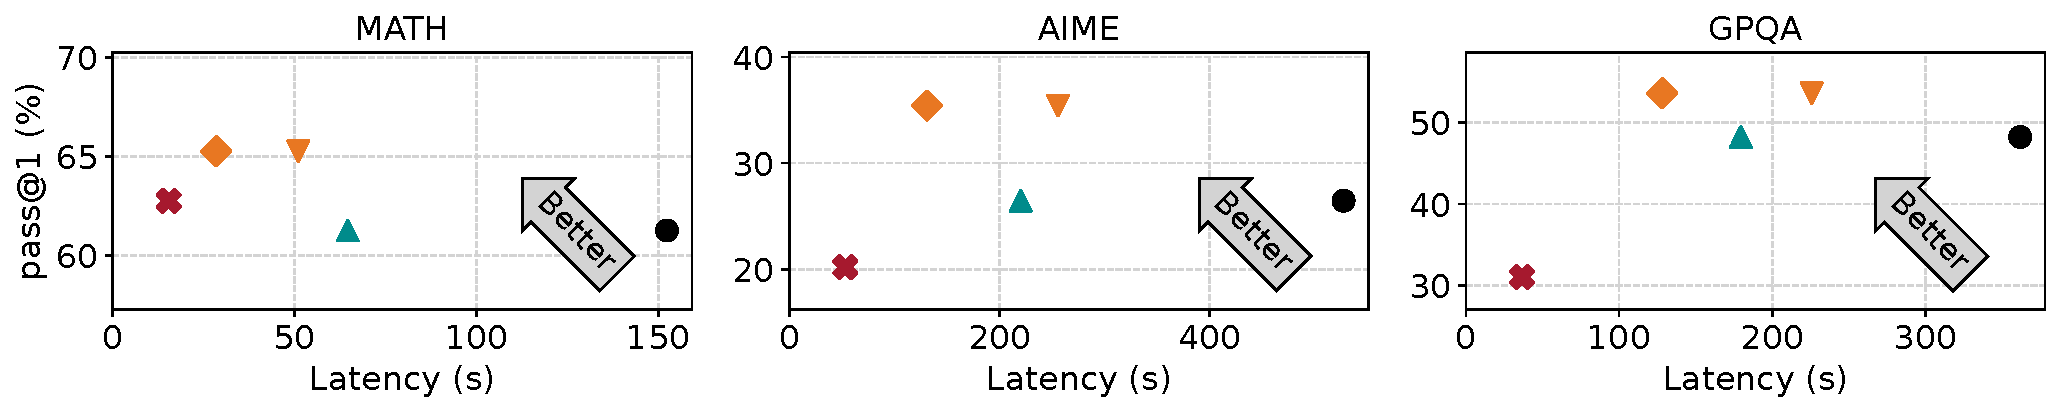
\includegraphics[width=0.99\textwidth]{figures/main_results/Qwen-32B_Zyphra-1.5B.pdf}
        \vspace{-5pt}
        \caption{QwQ-32B + Zyphra-1.5B}
        \label{fig:main_results_2}
    \end{subfigure}
    \hfill
    \begin{subfigure}[b]{\textwidth}
        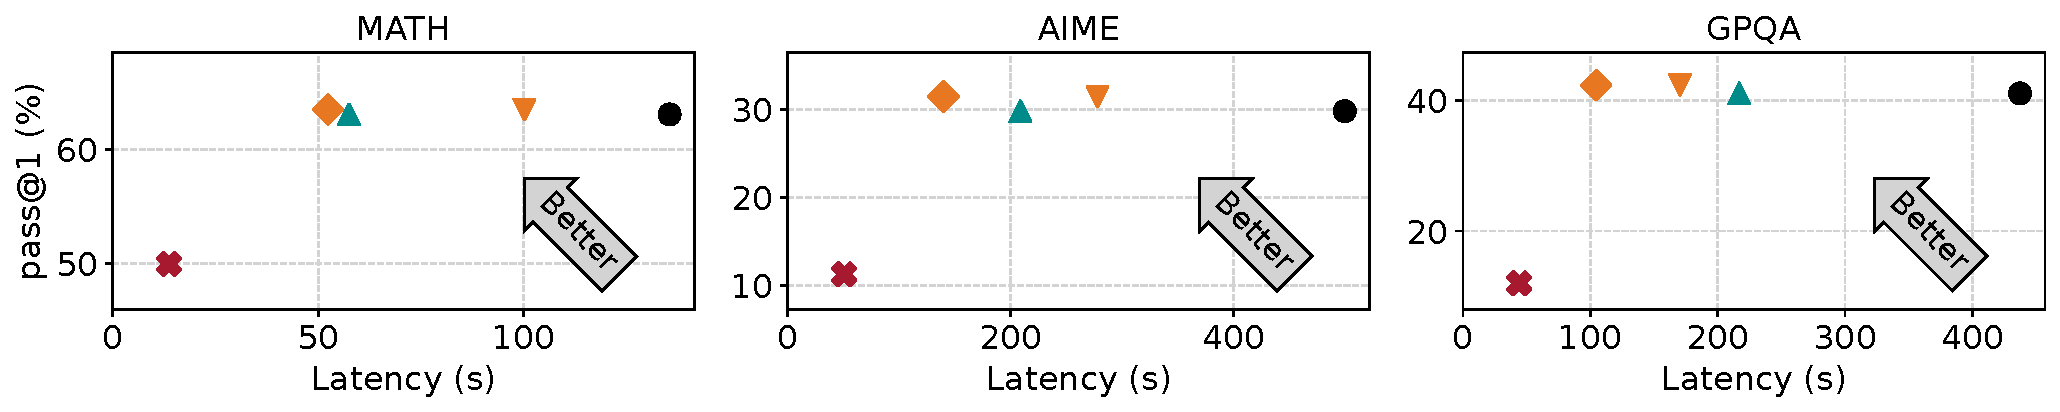
\includegraphics[width=0.99\textwidth]{figures/main_results/Skywork-Preview_deepseek-1.5B.pdf}
        \vspace{-5pt}
        \caption{Skywork-Preview-32B + R1-1.5B}
        \label{fig:main_results_3}
    \end{subfigure}
    \hfill
    \begin{subfigure}[b]{\textwidth}
        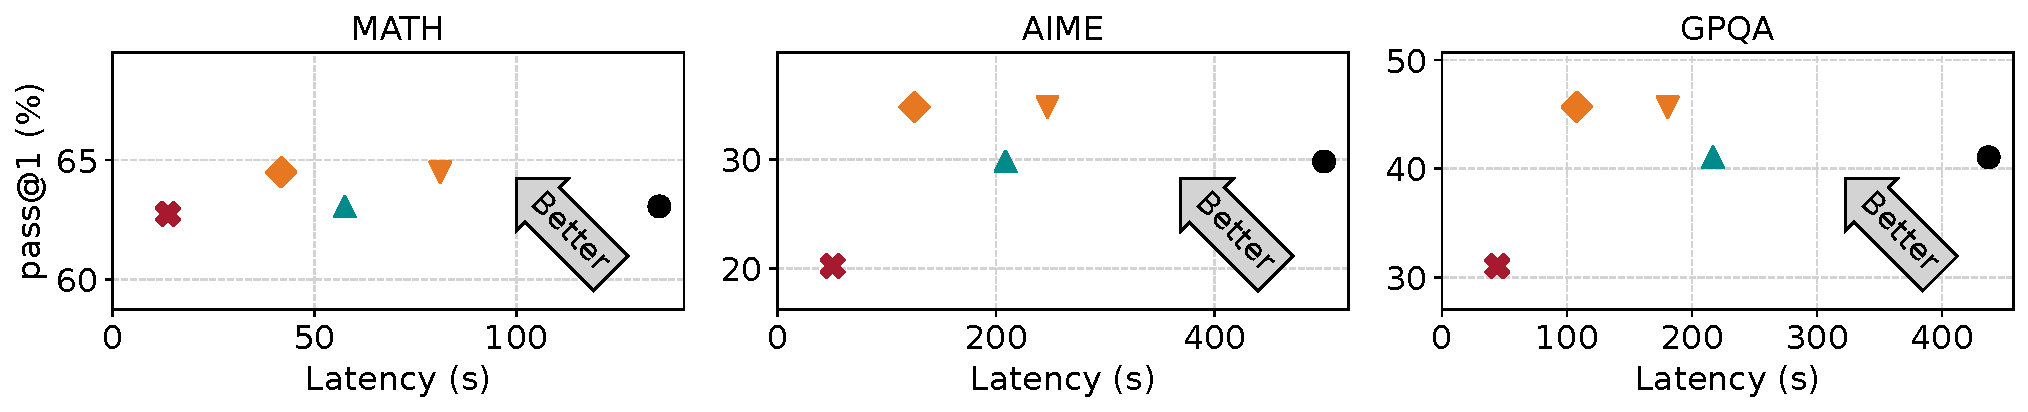
\includegraphics[width=0.99\textwidth]{figures/main_results/Skywork-Preview_Zyphra-1.5B.pdf}
        \vspace{-5pt}
        \caption{Skywork-Preview-32B + Zyphra-1.5B}
        \vspace{-5pt}
        \label{fig:main_results_4}
    \end{subfigure}
    \caption{Comparison of the accuracy and latency of different schemes on different model combinations. \name{} significantly reduces latency while improving accuracy over vanilla inference. When combined with speculative decoding, \name{} outperforms speculative decoding in both latency and accuracy on all datasets and model combinations.}
    \label{fig:main_results}
    \vspace{-15pt}
\end{figure}


\begin{figure}[t]
    \centering
    \begin{subfigure}[t]{0.5\textwidth}
        \centering
        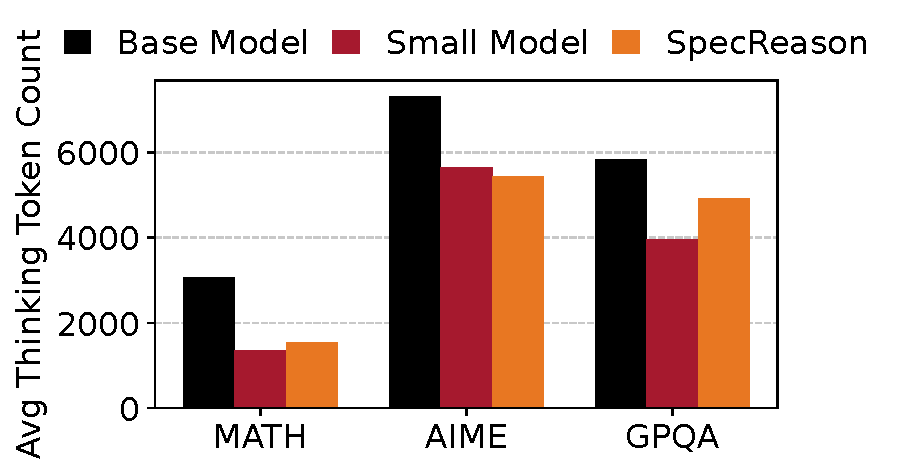
\includegraphics[width=\linewidth]{figures/acc_insight_len_Qwen-32B_Zyphra-1.5B.pdf}
        \caption{Output length comparison. \name{} reduces the token consumption needed to answer queries by adopting speculated steps from small models that are less verbose.}
        \label{fig:output_len_comparison}
    \end{subfigure}
    \hfill
    \begin{subfigure}[t]{0.48\textwidth}
        \centering
        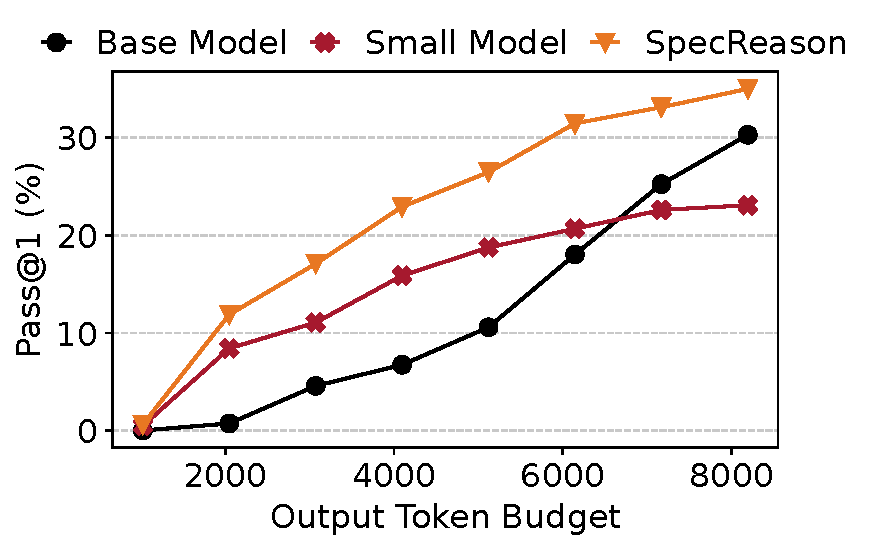
\includegraphics[width=\linewidth]{figures/acc_insight_linegraph.pdf}
        \caption{[AIME] Accuracy gap under different token budgets.}
        \label{fig:acc_by_seq_len}
    \end{subfigure}
    \caption{[QwQ-32B + Zyphra-1.5B] Intuition behind \name{}'s accuracy improvement. See Fig.~\ref{fig:acc_insight_len_all} in \S\ref{sec:appendix} for the full set of results.}
    \label{fig:acc_intuition}
\end{figure}

\begin{figure}[t]
    \centering
    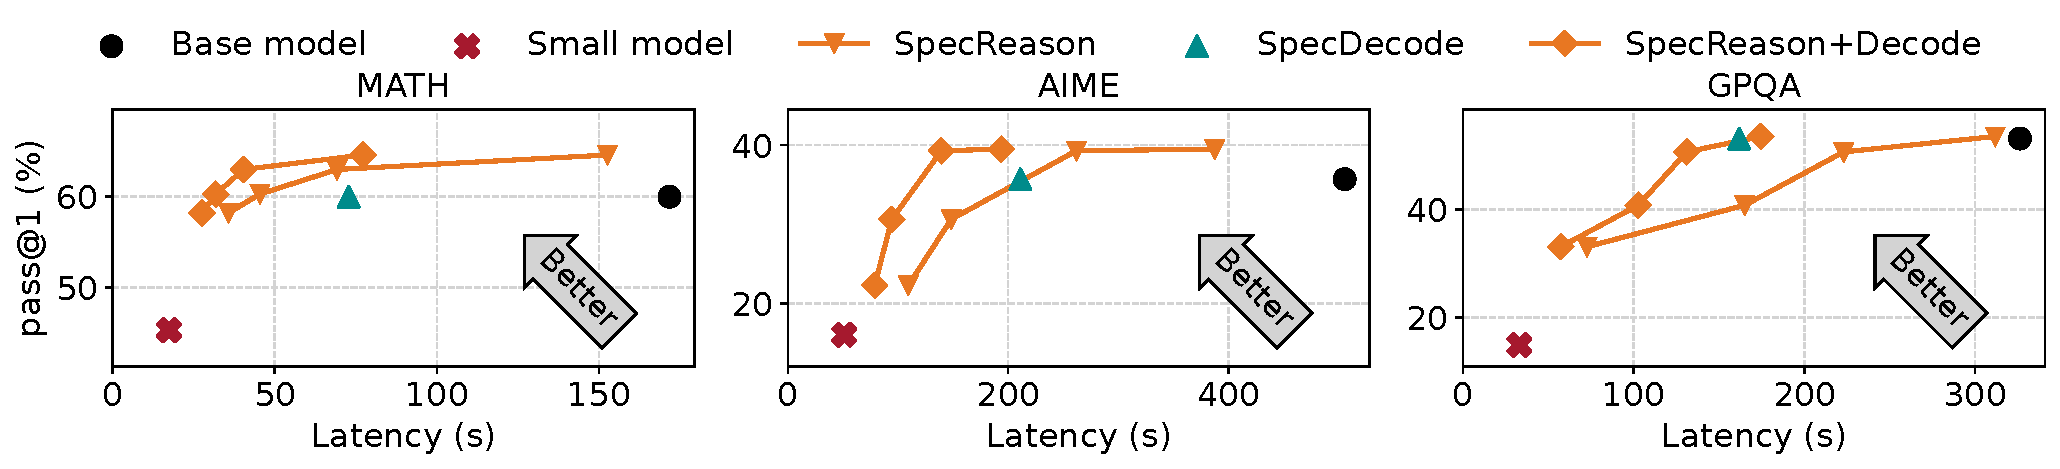
\includegraphics[width=0.99\textwidth]{figures/lat_acc_tradeoff.pdf}
    \caption{[QwQ-32B + R1-1.5B] \name{} allows trading off latency for accuracy via adjusting the acceptance threshold (from left to right, the thresholds are: 3, 5, 7, and 9 out of 9).}
    \label{fig:lat_acc_tradeoff}
    \vspace{-10pt}
\end{figure}



\subsection{Main Results}
\label{sec:main_results}

We compare \name{} against baseline methods in Fig.~\ref{fig:main_results}. Across the four model combinations, \name{} achieves a 1.5$\times$--2.5$\times$, 1.6$\times$--3.0$\times$, 1.4$\times$--2.5$\times$, 1.7$\times$--2.4$\times$ reduction in latency, respectively, compared to vanilla inference with the base model.   %

\textbf{Accuracy improvement.} Alongside these efficiency gains, \name{} also yields modest accuracy improvements of 1.3\%--3.6\%, 4.0\%--9.0\%, 0.4\%--1.7\%, and 1.4\%--5.0\% compared to the base model. The key reason behind this accuracy improvement is the reduction in token consumption required for reasoning. In Fig.~\ref{fig:acc_intuition}, we focus on the model combination with the highest overall accuracy improvement, QwQ-32B + Zyphra-1.5B, and compare the average number of thinking tokens needed to derive an answer between the base model, the small model, and \name{}. As seen in Fig.~\ref{fig:output_len_comparison}, the small model is generally less verbose than the base model, and because \name{} adopts many speculated steps from the small model, its token consumption is also reduced by 1.2$\times$--2.0$\times$. We also focus on the AIME dataset and vary the token budget to study its effect on the difference in accuracy between \name{} and the base model in Fig.~\ref{fig:acc_by_seq_len}. The effect of token reduction on accuracy is the most significant for tighter output token budgets (16.2\% at 4096 tokens) but shrinks as the base model is allowed to generate more thinking tokens (4.7\% at 8192 tokens). We also attribute these accuracy gains to \name{}’s explicit judgment and scoring mechanism at each reasoning step, which augments the model’s internal self-reflection with more structured assessment. 





When compared with speculative decoding, \name{} lies on the Pareto frontier of the accuracy-latency tradeoff. More importantly, combining \name{} with speculative decoding (\name{}+Decode) results in further latency reductions of 19.4\%--44.2\%, 30.8\%--58.0\%, 8.8\%--52.2\%, and 25.1\%--51.8\% over speculative decoding alone.
The most significant performance gains for \name{} when the base model is QwQ-32B occur on the MATH dataset, where both models achieve relatively high accuracies and the capability gap between the small and base models is the narrowest. This makes intermediate steps easier for the small model to speculate correctly, increasing the acceptance rate of speculated steps and thereby lowering end-to-end latency. In comparison, Skywork-Preview-32B is slightly inferior at instruction following, so \name{} has to adopt a higher threshold to avoid an accuracy loss, reducing \name{}'s latency wins.

Finally, when comparing \name{}+Decode with \name{}, \name{}+Decode reduces latency by 1.7$\times$--1.9$\times$, 1.7$\times$--1.8$\times$, 1.6$\times$--2.2$\times$, and 1.6$\times$--2.1$\times$, demonstrating the difference in ease of speculation across varying tasks. On these three datasets, the ratio of steps carried out by small models in \name{} is 38.1\%--80.0\%, 36.5\%--71.3\%, 39.3\%--70.2\%, and 41.4\%--66.6\%, respectively.
















        
        





\subsection{Controlling the Accuracy-Latency Tradeoff}
\label{sec:acc_lat_tradeoff}

In Fig.~\ref{fig:lat_acc_tradeoff}, we illustrate how \name{} enables flexible control over the accuracy-latency tradeoff, using a representative, randomly selected subdataset from the full datasets in \S\ref{sec:main_results} on QwQ-32B + R1-1.5B for ease of evaluation. During the base model’s evaluation of each reasoning step, we vary the acceptance threshold for the utility score between 3, 5, 7, and 9, and report the resulting accuracy and latency.

On the MATH subdataset, increasing the acceptance threshold from 3 to 7 results in fewer speculative steps from the small model being accepted. This leads to a latency increase from 35.7s to 69.2s, while accuracy improves from 59.4\% to 63.7\%, due to tighter control over the approximation level of intermediate reasoning steps. Notably, the gap between SpecReason+Decode and SpecReason widens from 8.1s to 28.8s, since more reasoning steps are delegated to the base model, and SpecReason+Decode reduces only the base model’s decoding time compared to \name{}.

A similar trend is observed on the AIME and GPQA subdatasets: as the acceptance threshold increases from 3 to 7, latency grows from 109.4s to 261.9s and from 72.7s to 223.0s, and accuracy improves from 22.3\% to 39.3\% and from 33.1\% to 50.7\%. However, the accuracy degrades less gracefully as the threshold is relaxed compared to the MATH subdataset. This is because the small model exhibits a larger performance gap relative to the base model on AIME and GPQA, making aggressive acceptance of its speculative steps more costly in terms of accuracy.

In Fig.~\ref{fig:earlyforce_knob}, we also study the effect of the alternative knob, forcing the first $n$ reasoning steps to be decoded by the base model, on the accuracy-latency tradeoff. As we change $n$ from 0 to 10, 20, 30, and 40, \name{}'s accuracy increases from 33.2\% to 37.3\% while the latency increases from 270.4s to 292.6s, showcasing an alternative approach to improve accuracy with a slight increase in latency.









\begin{figure}[t]
    \centering
    \begin{minipage}{0.42\textwidth} %
        \centering
        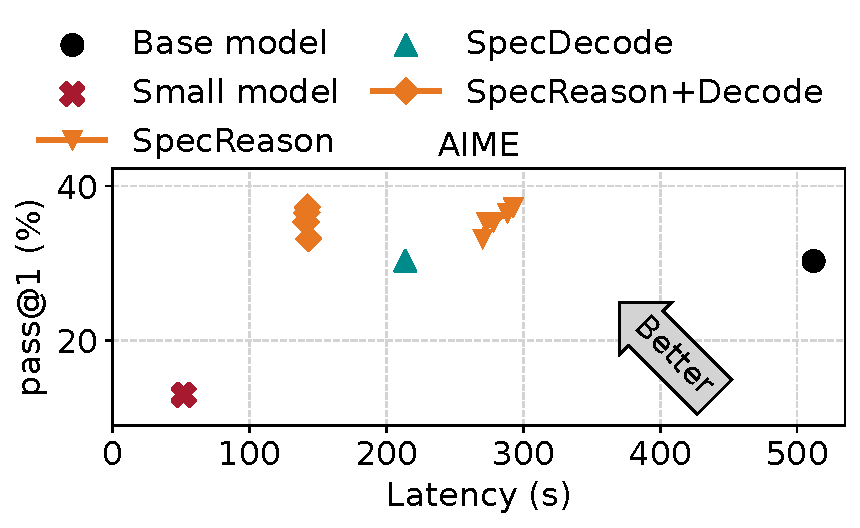
\includegraphics[width=\textwidth]{figures/lat_acc_tradeoff_earlyforce.pdf}
        \caption{Effect of the alternative knob: forcing the first $n$ steps for base model decoding.}
        \label{fig:earlyforce_knob}
        \vspace{-10pt}
    \end{minipage}
    \hfill %
    \begin{minipage}{0.55\textwidth} %
        \centering
        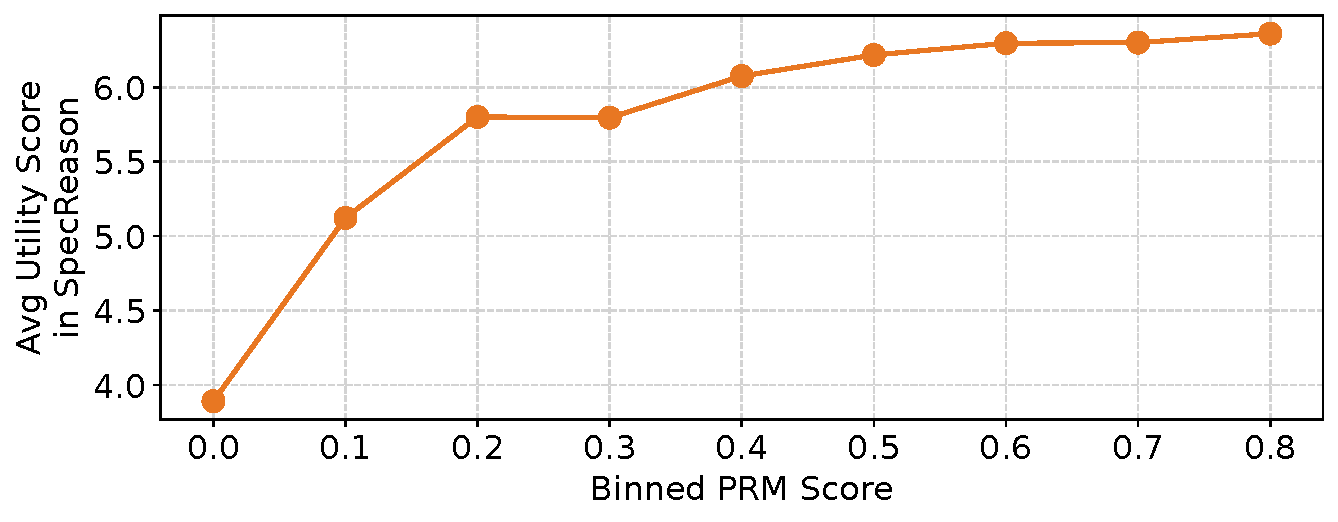
\includegraphics[width=\textwidth]{figures/prm_microbenchmark.pdf}
        \caption{The utility scores in \name{} closely reflect the quality score judgements from a process reward model. $x$ on the x-axis denotes PRM scores in the range $[x, x+0.1)$.}
        \label{fig:prm_microbenchmark}
    \end{minipage}
\end{figure}






























\subsection{Base Model's Judgement Capability}


The base model's ability to assess the quality of intermediate reasoning steps is a crucial cornerstone of \name{}'s performance. In this experiment, we compare the scores generated by a process reward model (PRM) -- which assigns a reward score to each step within the solution to a math problem -- with those given by the QwQ-32B base model on the AIME dataset. Specifically, we use Math-Shepherd~\citep{math_shepherd}, a PRM trained via reinforcement learning from the Mistral-7B base model on math problems, to score each speculated step produced by the R1-1.5B small model.

In Fig.~\ref{fig:prm_microbenchmark}, we bin the reward scores (a float from 0 to 1) into ten bins. Within each bin, we calculate the mean utility score given by the base model in \name{}. This analysis demonstrates a strong correlation between the base model's and the PRM’s assessments, particularly for lower-quality reasoning steps, where both models assign low scores. The results suggest that the base model can effectively approximate the PRM’s judgments, making it a viable option for evaluating reasoning step quality in \name{}.

